\documentclass{article}\usepackage[]{graphicx}\usepackage[]{color}
\graphicspath{ {./images/} }
% maxwidth is the original width if it is less than linewidth
% otherwise use linewidth (to make sure the graphics do not exceed the margin)
\makeatletter
\def\maxwidth{ %
  \ifdim\Gin@nat@width>\linewidth
    \linewidth
  \else
    \Gin@nat@width
  \fi
}
\makeatother

\definecolor{fgcolor}{rgb}{0.345, 0.345, 0.345}
\newcommand{\hlnum}[1]{\textcolor[rgb]{0.686,0.059,0.569}{#1}}%
\newcommand{\hlstr}[1]{\textcolor[rgb]{0.192,0.494,0.8}{#1}}%
\newcommand{\hlcom}[1]{\textcolor[rgb]{0.678,0.584,0.686}{\textit{#1}}}%
\newcommand{\hlopt}[1]{\textcolor[rgb]{0,0,0}{#1}}%
\newcommand{\hlstd}[1]{\textcolor[rgb]{0.345,0.345,0.345}{#1}}% 
\newcommand{\hlkwa}[1]{\textcolor[rgb]{0.161,0.373,0.58}{\textbf{#1}}}%
\newcommand{\hlkwb}[1]{\textcolor[rgb]{0.69,0.353,0.396}{#1}}%
\newcommand{\hlkwc}[1]{\textcolor[rgb]{0.333,0.667,0.333}{#1}}%
\newcommand{\hlkwd}[1]{\textcolor[rgb]{0.737,0.353,0.396}{\textbf{#1}}}%
\let\hlipl\hlkwb

\usepackage{framed}
\makeatletter
\newenvironment{kframe}{%
 \def\at@end@of@kframe{}%
 \ifinner\ifhmode%
  \def\at@end@of@kframe{\end{minipage}}%
  \begin{minipage}{\columnwidth}%
 \fi\fi%
 \def\FrameCommand##1{\hskip\@totalleftmargin \hskip-\fboxsep
 \colorbox{shadecolor}{##1}\hskip-\fboxsep
     % There is no \\@totalrightmargin, so:
     \hskip-\linewidth \hskip-\@totalleftmargin \hskip\columnwidth}%
 \MakeFramed {\advance\hsize-\width
   \@totalleftmargin\z@ \linewidth\hsize
   \@setminipage}}%
 {\par\unskip\endMakeFramed%
 \at@end@of@kframe}
\makeatother

\definecolor{shadecolor}{rgb}{.97, .97, .97}
\definecolor{messagecolor}{rgb}{0, 0, 0}
\definecolor{warningcolor}{rgb}{1, 0, 1}
\definecolor{errorcolor}{rgb}{1, 0, 0}
\newenvironment{knitrout}{}{} % an empty environment to be redefined in TeX

\usepackage{alltt}
\usepackage{listings}

\definecolor{mygreen}{rgb}{0,0.6,0}
\definecolor{mygray}{rgb}{0.5,0.5,0.5}
\definecolor{mymauve}{rgb}{0.58,0,0.82}

\lstset{ 
  backgroundcolor=\color{white},   % choose the background color; you must add \usepackage{color} or \usepackage{xcolor}; should come as last argument
  basicstyle=\footnotesize,        % the size of the fonts that are used for the code
  breakatwhitespace=false,         % sets if automatic breaks should only happen at whitespace
  breaklines=true,                 % sets automatic line breaking
  captionpos=,                    % sets the caption-position to bottom
  commentstyle=\color{mygreen},    % comment style
  deletekeywords={...},            % if you want to delete keywords from the given language
  escapeinside={\%*}{*)},          % if you want to add LaTeX within your code
  extendedchars=true,              % lets you use non-ASCII characters; for 8-bits encodings only, does not work with UTF-8
  firstnumber=1,                % start line enumeration with line 1000
  frame=single,	                   % adds a frame around the code
  keepspaces=true,                 % keeps spaces in text, useful for keeping indentation of code (possibly needs columns=flexible)
  keywordstyle=\color{blue},       % keyword style
  language=Python,                 % the language of the code
  morekeywords={*,...},            % if you want to add more keywords to the set
  numbers=left,                    % where to put the line-numbers; possible values are (none, left, right)
  numbersep=5pt,                   % how far the line-numbers are from the code
  numberstyle=\tiny\color{mygray}, % the style that is used for the line-numbers
  rulecolor=\color{black},         % if not set, the frame-color may be changed on line-breaks within not-black text (e.g. comments (green here))
  showspaces=false,                % show spaces everywhere adding particular underscores; it overrides 'showstringspaces'
  showstringspaces=false,          % underline spaces within strings only
  showtabs=false,                  % show tabs within strings adding particular underscores
  stepnumber=1,                    % the step between two line-numbers. If it's 1, each line will be numbered
  stringstyle=\color{mymauve},     % string literal style
  tabsize=2,	                   % sets default tabsize to 2 spaces
  title=\lstname                   % show the filename of files included with \lstinputlisting; also try caption instead of title
}

\usepackage{caption}
\usepackage{subcaption}

\title{LED Exercise}
\IfFileExists{upquote.sty}{\usepackage{upquote}}{}

\author{Kyle McCarty and Marc Los Huertos\footnote{Acknowledgments: Summer research students, Anna Burns and Alision Joseph contributed to these documents.}}


\begin{document}

\maketitle

\tableofcontents

\newpage

\section{Introduction}

The purpose of this document is to give a brief introduction and familiarization of the components that you will be using in your air quality station. It will also summarily discuss electrical circuits and software coding with the programming language Python.

\section{Components}

\subsection{General-Purpose Input/Output Pins (GPIO)}

\begin{itemize}

\item The general-purpose input-output pins (GPIO) are one of the main features that makes the Raspberry Pis so versatile. The pin header on the newer Raspberry Pis have 40 pins in total. We use these pins and connect them to devices to control them. In software, the GPIO pins can be designated either as an input pin or output pin.
\begin{figure}[h]
\begin{center}
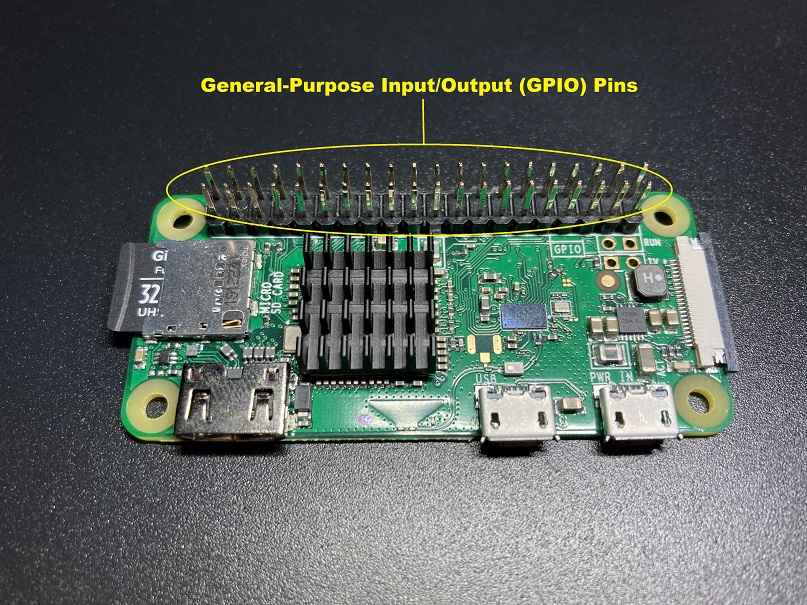
\includegraphics[width=1.00\textwidth]{pinheader}
\caption{Raspberry Pi Zero W board with pin header soldered on and labled.\label{fig:pinheader}}
\end{center}
\end{figure}
\item There are, however, a few pins that are not configurable. These are two 5 volt (5V) pins, two 3.3 volt (3V3) pins, and eight ground (0V) pins.
\begin{figure}
\begin{center}
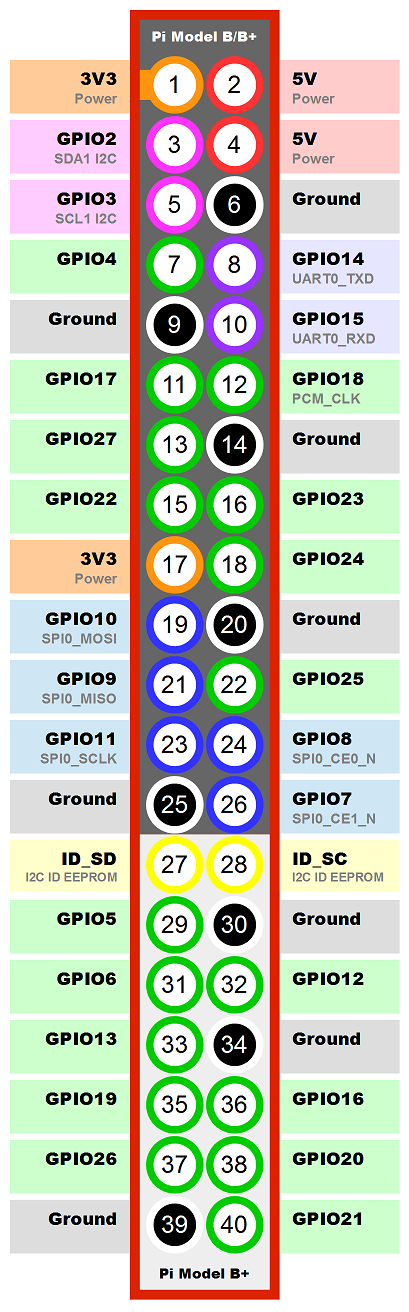
\includegraphics[width=0.50\textwidth]{GPIOlayout}
\caption{Diagram depicting the physical locations of each pin on the header, the software-assigned label, and function.\label{fig:GPIOlayout}}
\end{center}
\end{figure}
\item All of the other remaining pins are considered general purpose 3V3 pins. This means you can configure these pins as long as the input and outputs are 3V3.

\end{itemize}

\subsection{Jumper Wires}

\begin{itemize}
\item A jumper wire is a wire that is used to connect various electronic components. For example, a jumper wire will connect our Raspberry Pi to the breadboard, various components on the breadboard, and various sensors. These are usually found in a variety of colors, which can be tough to keep track of. However, red is almost always for the positive voltage and black is used for ground. It's highly recommneded to follow this convention -- could save much heartache.
\item It is also important to note, wires come in various shapes and sizes with different end connections. For example, you were supplied with wire that has two bare ends and wire that has one female connector and one male connector. You were supplied these two different wires to use the bare wires on the breadboard and the female/male connectors for the GPIO pins on the Raspberry Pi to the breadboard.

\begin{figure}[h]
\begin{center}
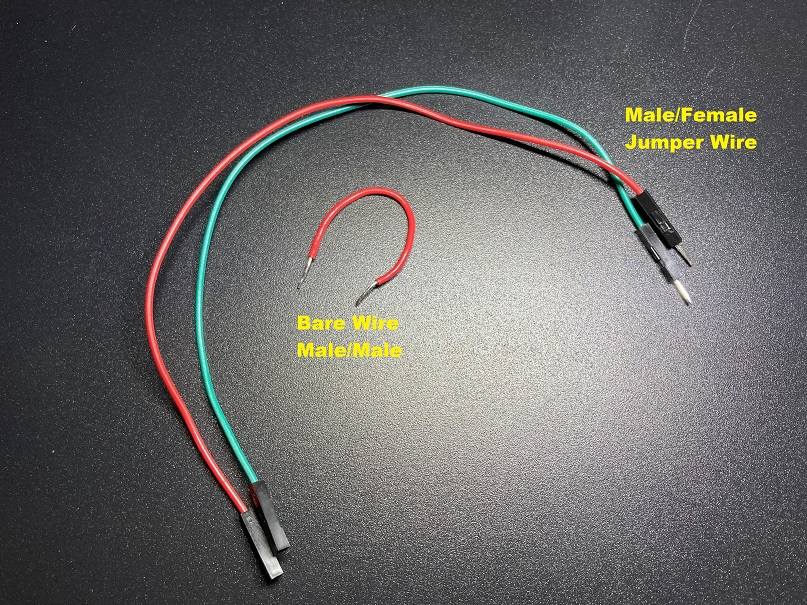
\includegraphics[width=0.90\textwidth]{wires}
\caption{Examples of two types of wire. Bare, male/male wire and male/female jumper wire.\label{fig:wires}}
\end{center}
\end{figure}
\end{itemize}

\subsection{Breadboard}

\begin{itemize}
\item Breadboards are testing platforms to build circuts. The have rows and columns which are electrically connected to give design flexibility. 
\item There are usually two or four rails or bus strips on the long sides of the board that are for power, in our case 3.3 volts or 5 volts, which is usually indicated by a red line. These buses are just a column or row, depending on breadboard orientation, of holes that are electrically connected. 
\item The ground, usually adjacent to the power bus, is usually blue or black colored. 
\item The rows in the inside are electrically connected, with a break in the center line. The center line is often strattled by a DIP (dual in-line package), so you can connect to each of the pins from both sides of the breadboard independently. 
\begin{figure}[h]
\begin{center}
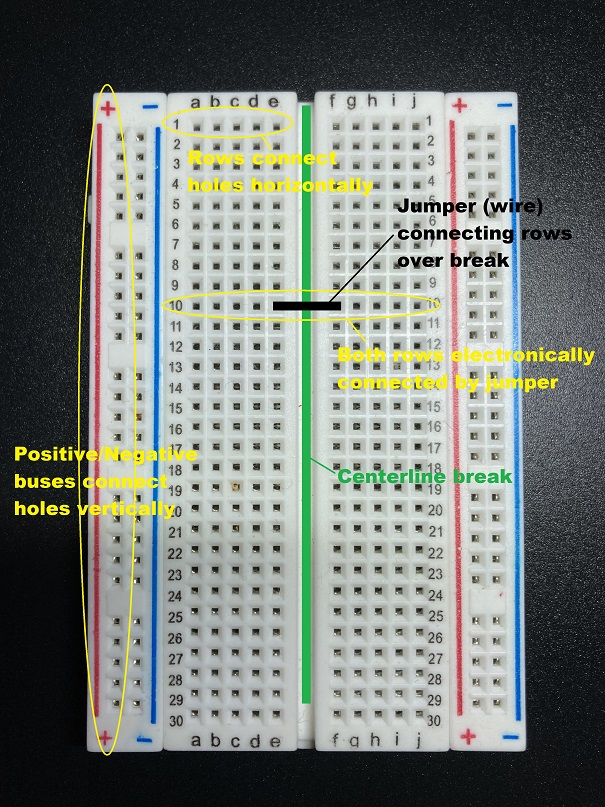
\includegraphics[width=0.60\textwidth]{bb2}
\caption{Breadboard illustration showing \textbf{+/-} columns are electrically connected while inside rows, with number-letter coordination, are electrically connected albeit being segregated at the centerline.\label{fig:bb2}}
\end{center}
\end{figure}
\end{itemize}

\subsection{LED}

\begin{itemize}
\item As many of you may know, a light emitting diode (LED) is a diode that emits light when voltage is applied to it. They come in many different colors and sizes, but for this exercise we are using relatively small LEDs.
\item LEDs actually have some requirements to work. We need to consider its polarity, forward voltage, and maximum current rating. Luckily, we have selected the right components for your already to use with the Raspberry Pi so you don't have to worry about that!
\item We will be using the Raspberry Pi to supply power to the LED so it will turn on. You will also be wiring in a resistor to make sure you don't burn your Raspberry Pi up.
\begin{figure}[h]
\begin{center}
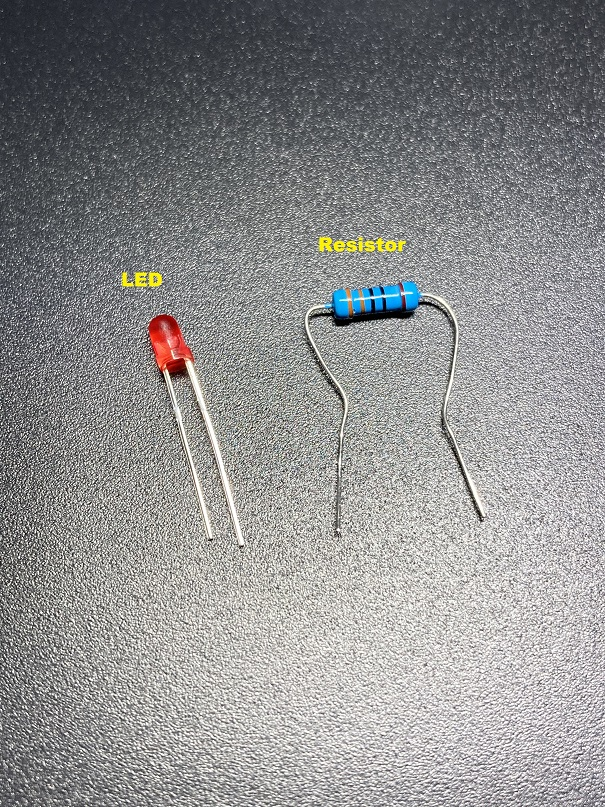
\includegraphics[width=0.65\textwidth]{ledres}
\caption{LED and resistor. The LED has two differently sized legs; forward voltage is applied to the LED's long leg. The colored bands on the resister are used to identify the amount of resistance, which is measured in ohms.\label{fig:ledres}}
\end{center}
\end{figure}
\end{itemize}

\subsection{Resistor}

\begin{itemize}
\item You must \textbf{always} use a resistor when wiring an LED to the Raspberry Pi. If you don't use one, you could potentially damage your Raspberry Pi.
\item A resistor limits the amount of electricity, or more specifically, current through a circuit. Resistance is measured in Ohms, and the larger the value, the more it limits current to flow.

\end{itemize}

\section{Wiring}

\subsection{Simple LED Circuit -- LED Always On}

We are going to create a simple circuit withe the LED using thing Raspberry Pi as a power source. This is really easy and will let you know if you understand how to wire a circuit. The LED should turn on as soon as you power on the Raspberry Pi!

\begin{enumerate}
\item First setup you power and ground jumper wires coming from your Raspberry Pi to your breadboard. Use your GPIO pinout diagram to figure out which pin is your 3.3 volt power and which pin(s) are ground. Connect your red wire's (color doesn't really matter but may help) female end to 3.3 volts power on the Raspberry Pi and the male end to the power/postive/+ bus on the breadboard (Figure~\ref{fig:pwrgrd}). It doesn't really matter which spot on the bus you connect it to, the whole column is connected, remember? Do the same for the ground jumper wire.

\begin{figure}[h]
\begin{center}
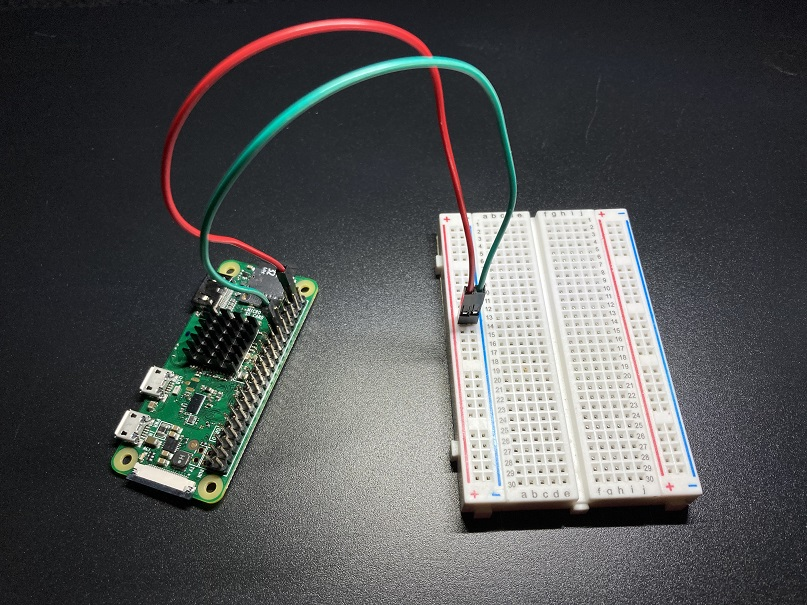
\includegraphics[width=0.75\textwidth]{pwrgnd}
\caption{Power and ground connection to breadboard and Pi.]{GPIOlayout}\label{GPIO}}
\end{center}
\end{figure}

\item Next setup the resistor on the breadboard. The resistor should be setup connecting the ground bus on the breadboard to an inside row. Keep in consideration you'll need at least one hole for the LED leg to connect in the same row (Figure~\ref{fig:res}). Resistors are not directionally dependant, so it doesn't matter which end of it is connected to the ground bus and which end is connected to the inside row.
\begin{figure}[h]
\begin{center}
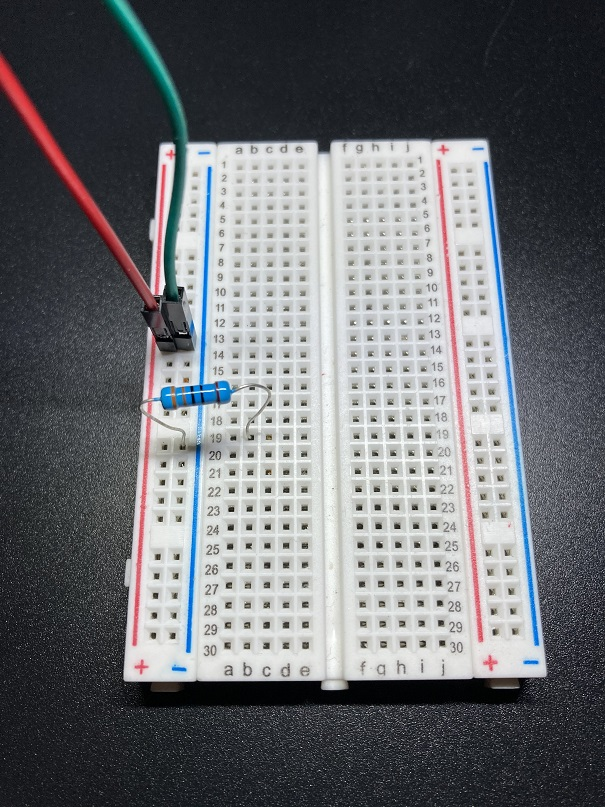
\includegraphics[width=0.65\textwidth]{res}
\caption{Resistor attached to breadboard.\label{fig:res}}
\end{center}
\end{figure}

\item Third, you need to connect the LED to the inside row the resistor is on and a \textbf{different} row. LEDs \textbf{are} directionally dependant. This is called polarity. If you notice, the LED has a short and long leg. Connect the shorter leg in the hole which is in the same row as the resistor. Connect the longer leg to a hole in another inside row (Figure~\ref{fig:bbledres}).

\item Lastly, connect a male/male wire from the longer leg of the LED to the power bus.

\item Now, double check your wiring and make sure it's right! It should look something like Figure~\ref{fig:bbresledwire}.


\begin{figure}
  \captionsetup{margin=10pt}
\begin{minipage}{.5\textwidth}
  \centering
  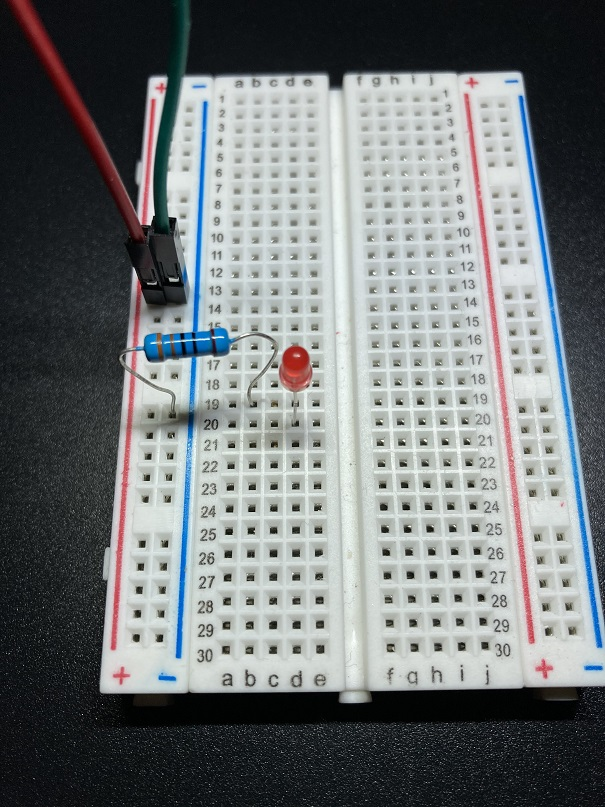
\includegraphics[width=\textwidth]{bbledres}
  \caption{LED and resistor attached to breadboard.}
  \label{fig:bbledres}
\end{minipage}%
\begin{minipage}{.5\textwidth}
  \centering
  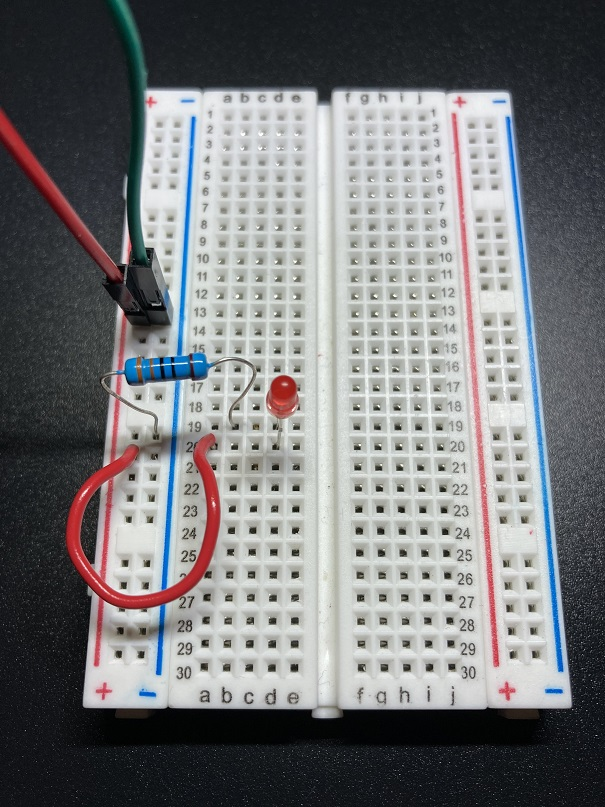
\includegraphics[width=\textwidth]{bbresledwire}
  \caption{All components hooked up in a complete circuit.}
  \label{fig:bbresledwire}
\end{minipage}
\end{figure}

\item Turn on your Raspberry Pi, and as soon as you do this, you should see your LED turn on!

\begin{figure}[!h]
\centering
\begin{subfigure}{.5\textwidth}
  \centering
  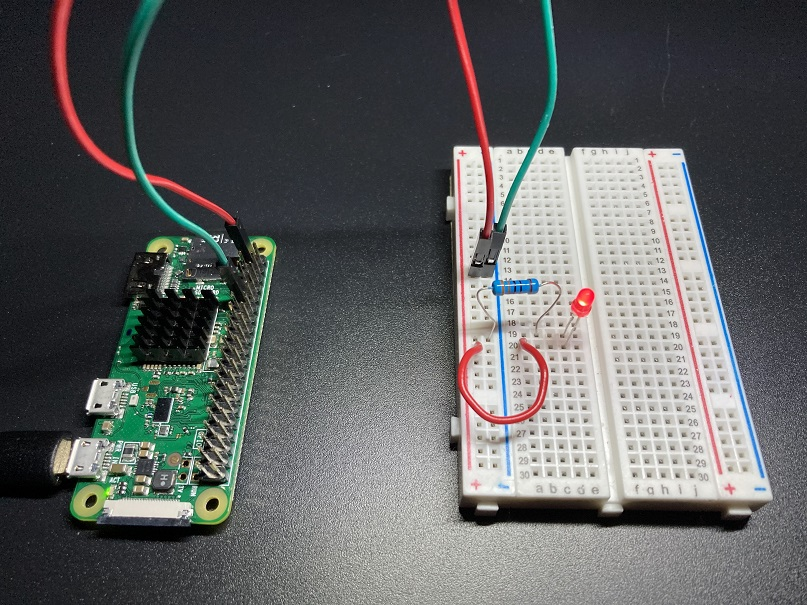
\includegraphics[width=1\linewidth]{ledon_bright}
  \label{fig:ledon_bright}
\end{subfigure}%
\begin{subfigure}{.5\textwidth}
  \centering
  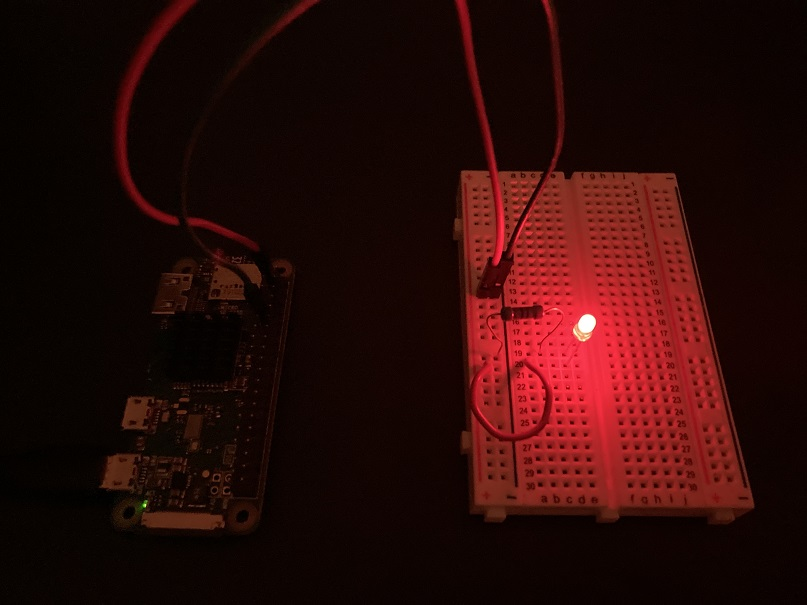
\includegraphics[width=1\linewidth]{ledon_dark}
  \label{fig:ledon_dark}
\end{subfigure}
\caption{LED is on!}
\label{fig:ledon}
\end{figure}

\item If your LED is not turning on, but you are sure you have your wiring correct, check the \textbf{troubleshooting} section below.
\end{enumerate}

\subsubsection{Simple LED Circuit Troubleshooting}
Help! My LED won't turn on!
\begin{itemize}
\item Triple check your wiring. Make sure the electrical components are all seated well on, or in, their GPIO pins or breadboard holes.
\item It is possible that you wired your LED in reverse (remember polarity). Try switching the leg positions.
\item Check your ground wire and its corresponding pin on the Raspberry Pi. Rarely a ground pin will not work. There are several ground pins on the Raspberry Pi, so try connecting the ground wire to a different ground GPIO pin.
\item Try switching out the LED. It is possible the LED is broken, this is why we gave you two LEDs.
\end{itemize}

\subsection{GPIO LED Circuit}
Next, we are going to change the wiring of the circuit to add a layer of complexity to this exercise. We are going to execute some Python code so that that LED blinks on and off.
\begin{itemize}
\item The first step to this is the use a GPIO pin, that isn't direct power, to send a signal that will turn on the LED and then another signal that will turn it off.
\item The Raspberry Pi communicates these signals in 2-logic levels, logical high signals or logical low signals. In this case, the Raspberry Pi will send a 3.3 signal, logic level high, or a 0V signal, logic level low. Obviously, 3.3 volts will turn on the LED and 0V will turn it off (no power supplied anymore).
\item The wiring essentially stays the same for this setup except that instead of connecting power to the constant 3.3 volt GPIO pin, connect it to \textbf{GPIO pin 24.} Refer to your GPIO pin diagram \ref{fig:GPIOlayout}.
\end{itemize}
\textbf{BE CAREFUL} there are two different naming conventions for the GPIO pins. The numbers within the circle on your pinout diagram (1-40) are the \textbf{physical} pin locations. The labels on the outside are the \textbf{BCM}, or \textbf{manufacture}'s designated nomenclature, GPIO 24 etc. You'll run into this issue when trying to code in Python. \label{GPIO24}

\section{Flashing LED}

\subsection{Using code to control the LED}

In order to instruct the Raspberry Pi to tell the LED to do more complicated things like turning off and on, we have to communicate with it in the form of a programming language and we'll use Python.

\subsection{What is Python?}

\textbf{Python} is a general-purpose programming language which its design philosohpy emphasizes readability of code.
\newline
\newline
In order to communicate instructions via Python, we need to write the code. We do this simply by using a text editor, or some kind of integrated development environment (IDE) like \textbf{Thonny}, for example. Thonny is the IDE that comes with Raspberry Pi OS.
\newline
\newline
A few notes on Python code:

\begin{itemize}
\item All the Python code you will be generating will have the file extension of \textbf{``.py''}.
\item Pay very close attention to spacing and indentations! This is very, very important in Python. Python uses particular formatting that represent ``code blocks.'' The code will not run if the indentations are at all off.
%- This code will automatically create a csv file under the title "pms5003_data.csv".  You can access this document in your Pi's File Explorer under "Pi".  
%When you go to open the csv file that the data stores to, select the following viewing settings for the most user-friendly experience:  tab, comma, trim spaces, and other (within the text box for other, type ")").  This will separate the actual values from the titles; you can do the rest of the "beautifying" of the data in R.
\end{itemize}

\subsection{Make your LED flash}

\begin{enumerate}
\item First, make sure you have connected your LED to the correct GPIO pin as decribed in \textbf{\ref{GPIO24}}. NOTE: This is not the 24th PIN -- look carefully that you are using PIN 14.
\item Boot up you Raspberry Pi and open the IDE Thonny.
\item Once you are in Thonny, write the following code: \newline
\lstinputlisting{../code/led.py}
\begin{itemize}
\item Keep in mind all of the syntax when you are writing the code. Python is sensitive to capitals, parenthesis, tabs, quotes, etc.
\end{itemize}
\item While writing the code, using Thonny, it will turn certain words into different colors or turn them bold, etc. This will help you recognize keywords of Python as well as syntax errors. For example, when you don't close your parenthesis, you will see the text highlighted gray. This is an advantage of writing code in an IDE.
\end{enumerate}

\section{Testing Your Code}
\begin{enumerate}
\item Next, we want to run the script! Press the big green \textbf{``Run''} button in the top toolbar of Thonny. Thonny may ask you to save the file. Go ahead and save it as something like \textbf{``ledflash.py''}.
\item If you see your LED flashing on and off, congratulations! You may stop the script anytime by pressing the big red \textbf{``Stop''} button in the top toolbar of Thonny.
\end{enumerate}

\subsection{Debugging}
\begin{enumerate}
\item If your light isn't flashing, you may have written the code incorrectly. Thonny is smart enough to read your code and point you in the direction of a suspected error. In the \textbf{``Shell''} tab you will see some red lettering that will describe where the error occured.
\item Don't forget to \textbf{``Stop''} the script if you need to make changes. If you don't stop the script, it won't allow you to edit.
\end{enumerate}

\end{document}
